% #############################################################################
% This is Chapter 5
% !TEX root = ../main.tex
% #############################################################################
% Change the Name of the Chapter i the following line
\fancychapter{Results}
%%%%%%%%%%%%%%%%%%%%%%%%%%%%%%%%%%%%%%%%%%%%%%%%%%%%%%%%%%%%%%%%%%%%%%%%
%                                                                      %
%     File: Thesis_Results.tex                                         %
%     Tex Master: Thesis.tex                                           %
%                                                                      %
%     Author: Francisco Azeredo                                        %
%     Last modified :  2 Jul 2015                                      %
%                                                                      %
%%%%%%%%%%%%%%%%%%%%%%%%%%%%%%%%%%%%%%%%%%%%%%%%%%%%%%%%%%%%%%%%%%%%%%%%
\label{chap:results}

This chapter validates the architecture and approaches developed in Chapter~\ref{chap:systemarch} through comprehensive experiments on document extraction, schema-aware retrieval, and agentic versus naive \gls{RAG} systems. We evaluate retrieval effectiveness across multiple datasets and measure answer quality using diverse similarity metrics.

\section{Information Extraction and Document Structuring}

Multiple multimodal models were tested for information extraction: PrimaLayout and PubLayNet showed promise but were insufficiently trained and produced unpredictable results. Nougat, an OCR engine that preserves document hierarchy in Markdown format, was selected for cases where PDFs lack embedded text metadata.
\section{Weaviate Schema: Case Study}
\label{sec:schema_example_study}

This section presents a concrete case study demonstrating how the Weaviate schema \ref{fig:weaviate_class} enables semantic search that respects and leverages the existing organizational structure,rather than treating documents as isolated items. The organizational model follows the UML in Figure~\ref{fig:weaviate_class}, with classes \textit{Fluxo} (workflow), \textit{Etapa} (stage), \textit{Entidade} (entity), \textit{Pasta} (folder), \textit{Ficheiro} (file), and \textit{Metadados} (metadata). The goal is twofold:

\begin{itemize}
    \item \textbf{Structure-aware retrieval:} Queries can traverse relationships (e.g., workflow \(\rightarrow\) stages \(\rightarrow\) files) and return results grounded in that hierarchy.
    \item \textbf{Semantic augmentation:} Each class embedded as vectors so that hybrid search (lexical + semantic) can surface relevant objects even when exact keywords or IDs are unknown.
\end{itemize}

\subsection{Objective and Use Case}

This case study demonstrates structure-aware semantic search by considering a corporate repository with approvals and contracts organized by entity and folder, and operational progress tracked as workflows with stages. A query for "contract approvals" should: (1) identify relevant workflows and stages, (2) traverse to file objects within the appropriate folders and entities, and (3) surface associated metadata. This aligns with organizational requirements where context (ownership, location, workflow progress) is as important as document content.

\subsection{Implementation Details}

The schema instantiates six collections—Fluxo, Etapa, Entidade, Pasta, Ficheiro, Metadados—each with a textual property (e.g., name) vectorized via transformer encoding for semantic indexing. Named vectorization supports hybrid retrieval by combining semantic scoring with graph traversal. Generative integration through Ollama and embeddings from sentence-transformers/all-MiniLM-L6-v2 supports grounded responses when appropriate.

\noindent\textbf{Cross-References (from UML)}\\
References implement the hierarchy and traversal paths and are formed directly from the UML diagram in Figure~\ref{fig:weaviate_class}. They define the possible navigation paths starting from each object/class:
\begin{itemize}
    \item \textit{Fluxo} \(\rightarrow\) \texttt{hasEtapas}, \texttt{belongsToFicheiros}, \texttt{belongsToPastas}.
    \item \textit{Etapa} \(\rightarrow\) \texttt{belongsToFluxo}, \texttt{hasFicheiros}.
    \item \textit{Entidade} \(\rightarrow\) \texttt{hasPastas}, \texttt{hasFicheiros}.
    \item \textit{Pasta} \(\rightarrow\) \texttt{hasEntidades}, \texttt{hasFluxos}, \texttt{hasFicheiros}.
    \item \textit{Ficheiro} \(\rightarrow\) \texttt{belongsToMetadados}, \texttt{hasEtapas}, \texttt{hasPastas}, \texttt{hasEntidades}.
    \item \textit{Metadados} \(\rightarrow\) \texttt{hasFicheiros}, \texttt{hasEtapas}, \texttt{hasPastas}, \texttt{hasEntidades}.
\end{itemize}
These references allow queries to traverse from workflows to stages to files, or from entities to folders to files and their associated metadata.

\noindent\textbf{Sample Data and Tests}
To validate the schema, synthetic data was inserted across classes with consistent linking (e.g., multiple \textit{Entidade}, each with several \textit{Pasta}, each with multiple \textit{Ficheiro}, each with \textit{Metadados}; plus several \textit{Fluxo} with many \textit{Etapa}). The following test queries illustrate structure-aware and semantic retrieval:
\begin{itemize}
    \item \textbf{Fluxo \& Etapas:} Fetch \textit{Fluxo} objects with their \textit{Etapa} names to verify workflow-stage traversal.
    \item \textbf{Entidade hierarchy:} Fetch \textit{Entidade} with nested \textit{Pasta} \(\rightarrow\) \textit{Ficheiro} \(\rightarrow\) \textit{Metadados} to demonstrate hierarchical expansion.
    \item \textbf{Global semantic search:} Run a hybrid search across all collections for a free-text query (e.g., “contract approvals”) and sort results by semantic score, showing how relevant objects are surfaced even when exact locations or identifiers are unknown.
\end{itemize}

\subsection{Discussion and Key Findings}
This example shows that vector databases like Weaviate can support company semantic retrieval that is \textit{aware of organizational structure}. By aligning collections and references with the UML model and enriching each node with embeddings, the system produces \textbf{explainable results} (returned items include their position in the hierarchy—e.g., which entity/folder/workflow they belong to—and their linked metadata), \textbf{flexible navigation} (agents or users can start from any node—workflow, entity, file—and traverse to related items), and \textbf{robust querying} (hybrid search compensates for inconsistent terminology while references maintain precise relationships).
In practice, this approach supports agentic retrieval flows that combine semantic ranking with graph-like traversal, improving precision and user trust when working within complex corporate repositories.


\section{Metadata Extraction versus Naive RAG}
\subsection{LiHua-World Dataset}
\label{subsec:LiHua-World}
The knowledge graph experiment uses the \emph{LiHua-World} corpus: a time-indexed set of short textual records organized into weekly folders (e.g., \path{week11/20260318_1510.txt}) and topical subfolders (e.g., \path{bakery_deliver/20260531.txt}). Each file contains concise, structured messages or notes about daily events (meetings, deliveries, fitness plans, chats, travel, garden updates), often with implyingparticipants and locations. This format provides:
\begin{itemize}
    \item \textbf{Temporal signals:} timestamps encoded in filenames (YYYYMMDD\_HHMM) and dates inside texts, enabling ordering and interval reasoning.
    \item \textbf{Multi-actor context:} recurring names across files (e.g., Li Hua, Wolfgang, Jennifer) support relationship extraction.
    \item \textbf{Domain variety:} community garden, bakery deliveries, fitness training, entertainment, and travel, which stress-test entity and relation typing.
\end{itemize}

\subsection{Knowledge Graph Ingestion Pipeline}

The corpus is processed through the metadata extraction framework by performing: (1) \textbf{Entity extraction:} using LLM-guided prompts to identify normalized entities (people, organizations, locations, events); (2) \textbf{Relation extraction:} inferring semantic relationships between entities based on proximity; (3) \textbf{Object creation:} creating  Weaviate objects for extracted entities with cross-references; (4) \textbf{Vectorization}:embedding textual properties for hybrid retrieval.


In this setup, answers were generated using sentence embedding model All-MiniLM-L6-v2 for retrieval and the local LLM Qwen2M for generation. The benchmark dataset consisted of 628 questions categorized as: (1) \textbf{Single}—direct factoid questions that can be answered from a single evidence source; (2) \textbf{Multi}—questions requiring multi-hop reasoning and/or temporal or causal understanding; (3) \textbf{Null}—questions with insufficient evidence.

The experiment compares knowledge-graph–aware retrieval (Mini and Light) against a naive baseline.
Figure~\ref{fig:Lihua-World} presents the results across all metrics.
\begin{figure}[H]
    \centering
    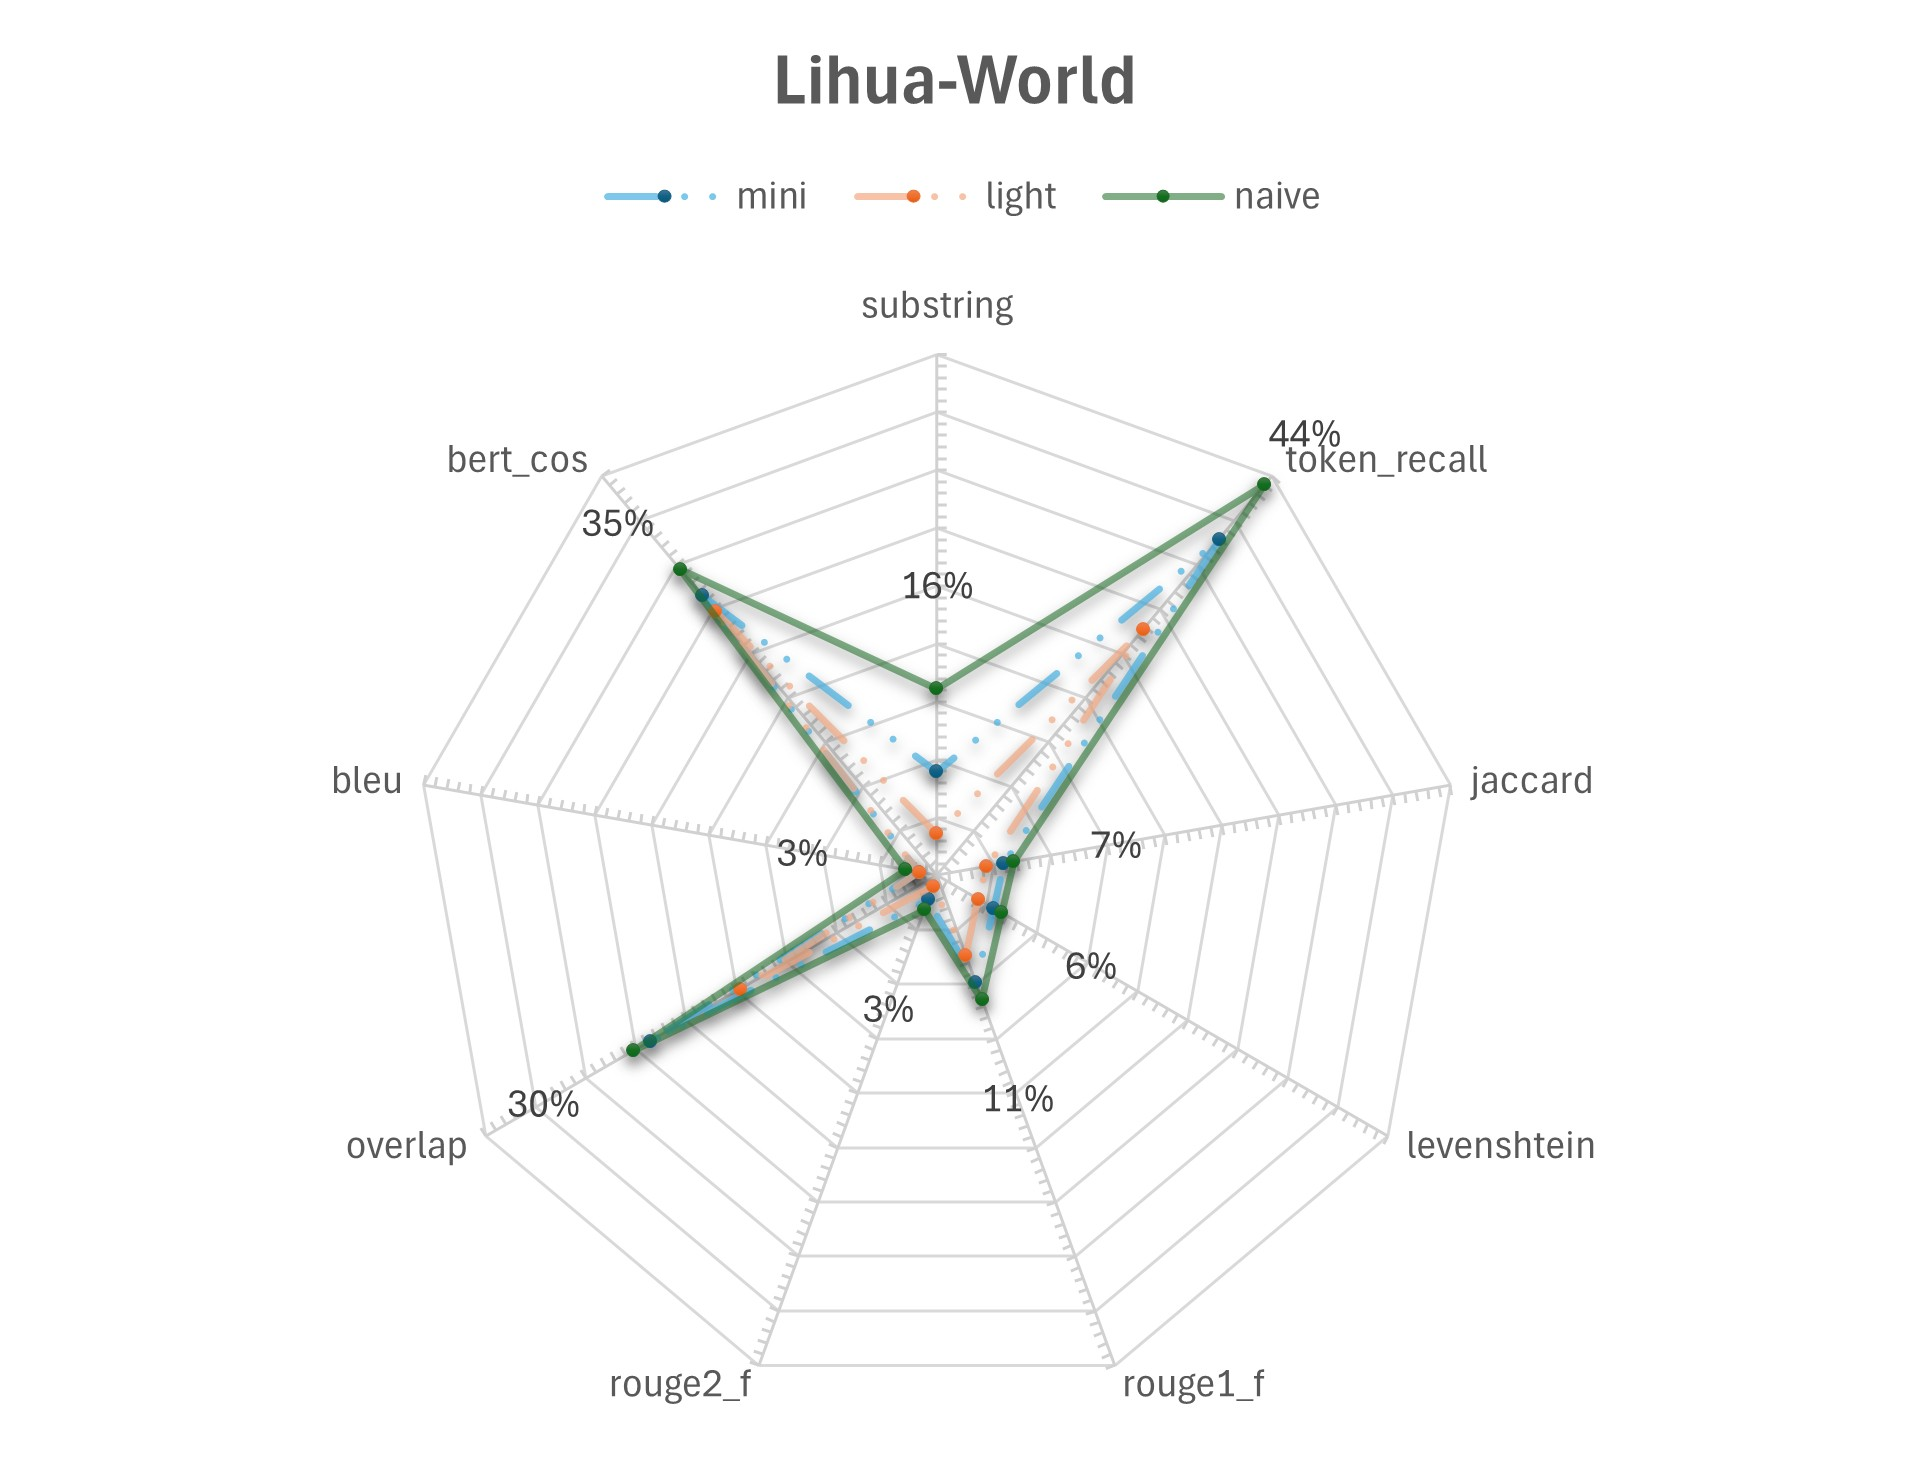
\includegraphics[width=1\linewidth]{Figures/Lihua-World.jpg}
    \caption{3 query types tested. With qwen2m as the \gls{LLM} and all-MiniLM-L6-v2 as embedding model}
    \label{fig:Lihua-World}
\end{figure}
Among the metrics, \textbf{Token Recall} achieved the highest score (44\%), and is the most relevant for this type of QA dataset.

\footnote{Note on metrics The full definitions and motivations for the evaluation metrics are provided in previous section \ref{sec:text-similarity-metrics}. Here we briefly reference the same set—lexical (Token Recall, Jaccard, Overlap), structural (Levenshtein, ROUGE, BLEU), and semantic (\gls{BERT} cosine)—and focus on interpreting the results in this experiment.}

\subsection{Semantic Similarity}
	\textbf{\gls{BERT} cosine similarity} score was moderate (35\%). This is largely due to length imbalance between short gold answers (sometimes a single token) and longer generated responses: sentence-level embeddings such as \textit{all-MiniLM-L6-v2} capture global semantics, so single-token vs. full-sentence comparisons tend to yield low cosine values.

\subsection{Lexical Accuracy}
	\textbf{Token Recall} (44\%) confirms that essential tokens are often present in predictions. The \textbf{Overlap Coefficient} (30\%) is comparatively robust to length differences, since it does not penalize extra tokens. In contrast, \textbf{Jaccard} (7\%) performs poorly when generated answers are longer, as the inflated union suppresses the overlap proportion—even for partially correct outputs.

\subsection{Structural Similarity}
	\textbf{Levenshtein} (6\%) provides a weak signal under large length differences. \textbf{ROUGE-1 F1} (11\%) and \textbf{ROUGE-2 F1} (3\%) partly mitigate this by balancing precision and recall over n-grams, although longer responses containing irrelevant tokens reduce precision. ROUGE-2 is particularly low because short gold answers rarely contain bigrams. Finally, \textbf{BLEU} (3\%)—originally designed for machine translation—over-penalizes deviations and brevity mismatches in this context, making it unsuitable for this task.

\subsection{Summary}
This experiment implemented an automated approach constructing a knowledge graph. The goal was to enable retrieval that leverages explicit entity relationships and organizational context rather than relying solely on surface-level text.

However, the results show that the current automatic knowledge graph construction fails to reliably produce a strong semantic structure for retrieval. In practice, direct embedding-based indexing using sentence transformers remains significantly faster, cheaper, and more effective for retrieval tasks, consistently outperforming the knowledge graph approach in this setup.

Profiling and structuring text with an LLM is also considerably more computationally expensive: each 200-token chunk is processed through a few-shot prompt (with many input tokens), up to three times, plus an additional pass for entity merging and summarization. This makes large-scale knowledge graph creation costly. While using a heavier LLM could improve the quality of the knowledge graph and its retrieval performance, the resource requirements and latency increase substantially.

In summary, while knowledge graphs offer richer structure and could become more competitive with stronger \glspl{LLM}, current embedding models provide a more scalable and efficient solution for semantic retrieval. Future work may revisit knowledge graph approaches as \glspl{LLM} costs decrease and capabilities improve.

\section{Naive versus Agentic RAG on Company Data}
\label{sec:expNaiveVsAgenticRAG}
This experiment aims to evaluate the effectiveness of an agentic retrieval-augmented generation (\gls{RAG}) approach compared to a naive \gls{RAG} baseline in answering context-specific questions about company information. The goal is to determine whether an agent that plans and reasons over retrieved documents can provide more accurate and relevant answers than a straightforward retrieval and generation pipeline.

For this experiment, a synthetic company QA dataset was created in two automated stages:
\begin{enumerate}
        \item \textbf{Document Generation:} First, a set of 1000 realistic administrative documents was generated using a \gls{GPT}-5 model. Each document was produced by prompting the model with a specific archival classification (from a public sector taxonomy), including its description, notes, and index terms, but instructing the model to never mention the class name in the content. The result is a diverse collection of plausible, well-structured company files, each corresponding to a different administrative or legal context. The total cost of generating these documents was around 5 dollars (around 10000 tokens per request).
        \item \textbf{QA Pair Generation:} \label{subsec:qa-generation} Next, for a random subset of these documents, a second generative model (also \gls{GPT}-5) was used to create question-answer pairs. The model was prompted with the full content of each document and instructed to generate a specific, contextual question that could only be answered by reading that document, along with a precise answer based exclusively on its content. This ensures that each QA pair is tightly coupled to a single file and cannot be answered from general knowledge or other documents. The cost of generating 300 such QA pairs was around 0.85 dollars.
\end{enumerate}

This process yields the \gls{QA} benchmark used to test developed \gls{RAG} systems, where each question is answerable only by retrieving the correct company file and reasoning over its content. The dataset is well-suited for evaluating (\gls{RAG}) systems, as it requires both accurate retrieval and grounded answer generation.

\subsection{Vector Database Setup}
The vector database used in this work is Weaviate. It is populated with 1000 synthetic company documents created earlier (see Section~\ref{sec:schema_example_study} and the dataset generation steps) and indexed using \textit{sentence-transformers/all-MiniLM-L6-v2} embeddings. The schema is simple: a single class \textit{Ficheiro} (file) with properties \texttt{text} and \texttt{file\_path}. Each document is stored as one object, with \texttt{text} vectorized (named vector \texttt{text\_vector}) to support semantic search; \texttt{file\_path} stores the document source for grounding answers. This same index is used by both the naive and agentic systems in the subsequent experiments.

\subsection{Naive RAG and CoT Baselines}
\label{sec:naive-rag-and-cot-baseline}
The naive baseline retrieved top-ranked passages from Weaviate and generated an answer; the CoT variant used the same retrieval with a short step-by-step hint.
For each question in the \gls{QA} dataset (generated in \ref{subsec:qa-generation}), the naive pipeline executes:
\begin{enumerate}
    \item Run a hybrid search in Weaviate (\(\alpha = 0.7\)) over \texttt{text\_vector} with the question to retrieve the top-$k$ objects containing \texttt{text} and \texttt{file\_path}.
    \item Generate a concise answer grounded in the retrieved content.
\end{enumerate}

At a high level, the naive pipeline performs a single retrieve-and-generate pass over hybrid search results in Portuguese. Variants with \texttt{qwen2.5} were tested to pick a cost-effective baseline, then the best was re-run with ChatGPT-5 to estimate an upper bound on quality. See Algorithm~\ref{alg:naive-weaviate-hybrid} (Appendix~B) for details.
The results are presented in Figure~\ref{fig:weaviate_test}.
This is used as a control: it is simpler to implement and requires no large model for planning.
\begin{figure}
    \centering
    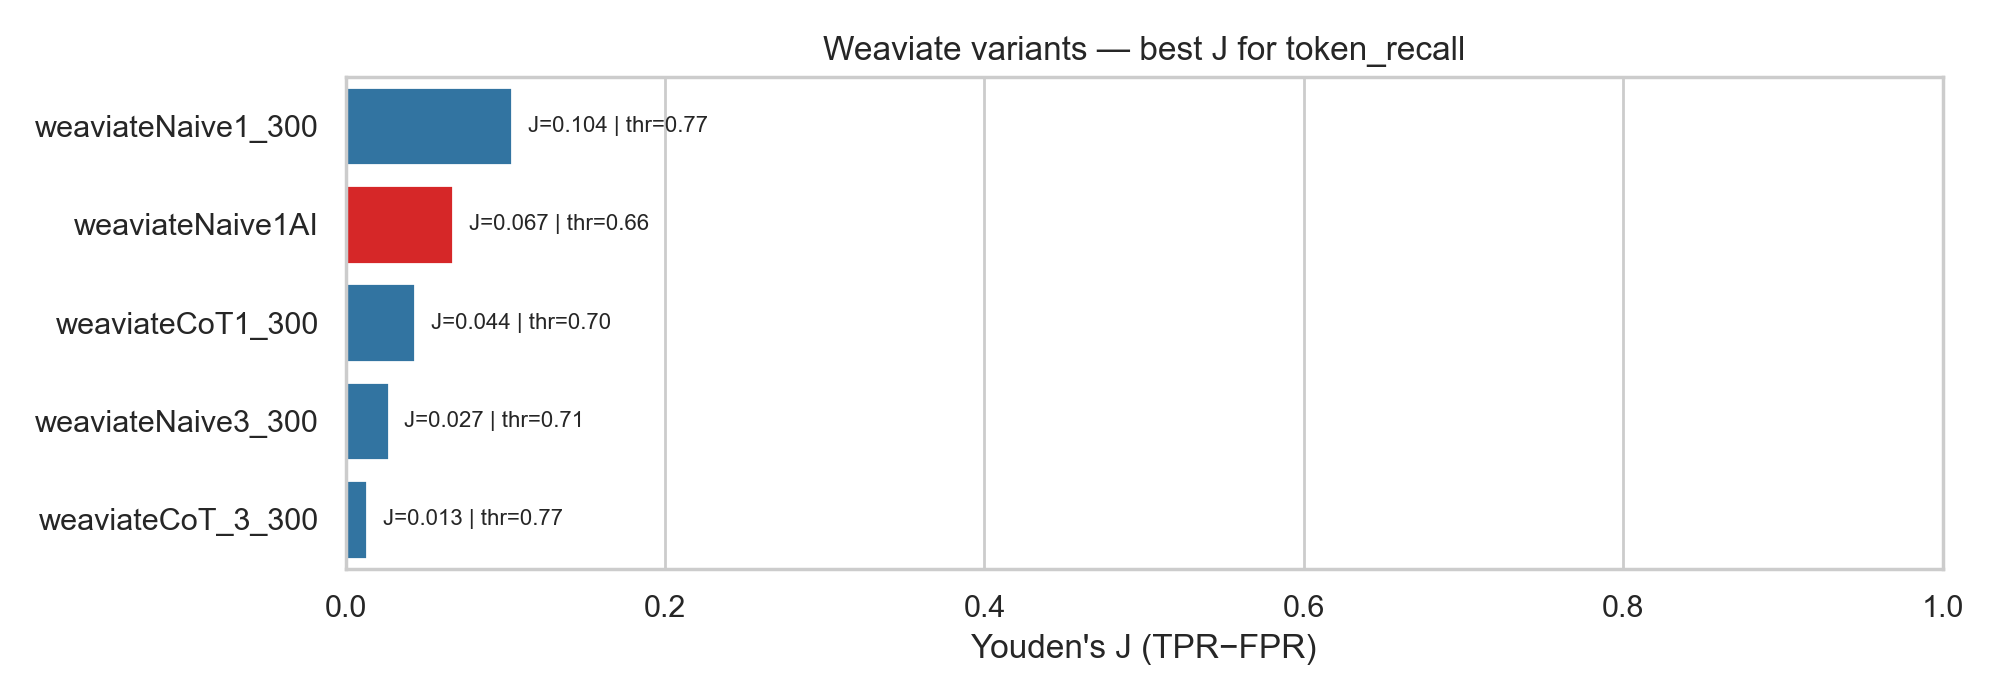
\includegraphics[width=1\linewidth]{Figures/10_weaviate_best_j_token_recall.png}
    \caption{Youden's J statistic for qualifying best naive \gls{RAG} variant. With qwen2.5m as the \gls{LLM} and all-MiniLM-L6-v2 as embedding model. And a chatgpt5 variant using best top-$k$ and prompt parameters.(k=4, prompt=naive)}
    \label{fig:weaviate_test}
\end{figure}
\subsection{Agentic RAG Setup}
\label{sec:agentic-test}

To set up the test, a \textbf{ReAct} agent was developed and connected to a Weaviate vector database via \gls{MCP} developed in this thesis~\ref{sec:weaviate-mcp-server}. Following initial trials with a local model (\texttt{qwen2.5m}) that exhibited frequent context drift—drifting from the question and leading to extractive outputs—reinforcing the need for a larger context window, \textbf{ChatGPT-5} was used for planning and generation, as a larger model is required to maintain multi-step reasoning within its context window.

\subsection{Agent Workflow}
For each question in the \gls{QA} dataset (generated in \ref{subsec:qa-generation}), the agent follows a ReAct loop:
\begin{enumerate}
\item \textbf{Plan:} Sketch a brief strategy to find the answer.
\item \textbf{Retrieve:} Fetch the most relevant documents.
\item \textbf{Observe \& Reflect:} Inspect the evidence and, if needed, refine the plan and retrieval.
\item \textbf{Answer:} Produce a concise response grounded in the retrieved content.
\end{enumerate}

Across \textbf{300} questions, the agent sometimes required up to \textbf{20} \gls{LLM} calls per question, with a total run cost of approximately \textbf{\$14}. Reasoning improves answer quality, but it significantly increases latency and cost compared to naive \gls{RAG}.

The cost-quality trade-off can be expressed as: achieving 60.4\% retrieval rate via agentic \gls{RAG} costs approximately \textbf{\$0.047 per question}, compared to \textbf{\$0.0017} for naive \gls{RAG} at 13.8\% retrieval. This \textbf{27.6x cost increase} yields a \textbf{4.4x improvement in retrieval accuracy}, representing a favorable trade-off for scenarios where accuracy is prioritized over cost.

\section{Evaluation of Quality Metrics}
\label{sec:metric-evaluation-quality}
To evaluate answer quality, the same metrics as in the previous experiment (Section~\ref{sec:expNaiveVsAgenticRAG}) are used, and the analysis proceeds a step further under the hypothesis that answers can only be correct if the source document is correctly retrieved. This is done by determining which threshold for a metric score to categorize an answer as correct aligns with the source being correctly retrieved. The optimal threshold maximizes Youden's J statistic, defined as the difference between true positive rate (TPR) and false positive rate (FPR).
\begin{figure}[H]
    \centering
    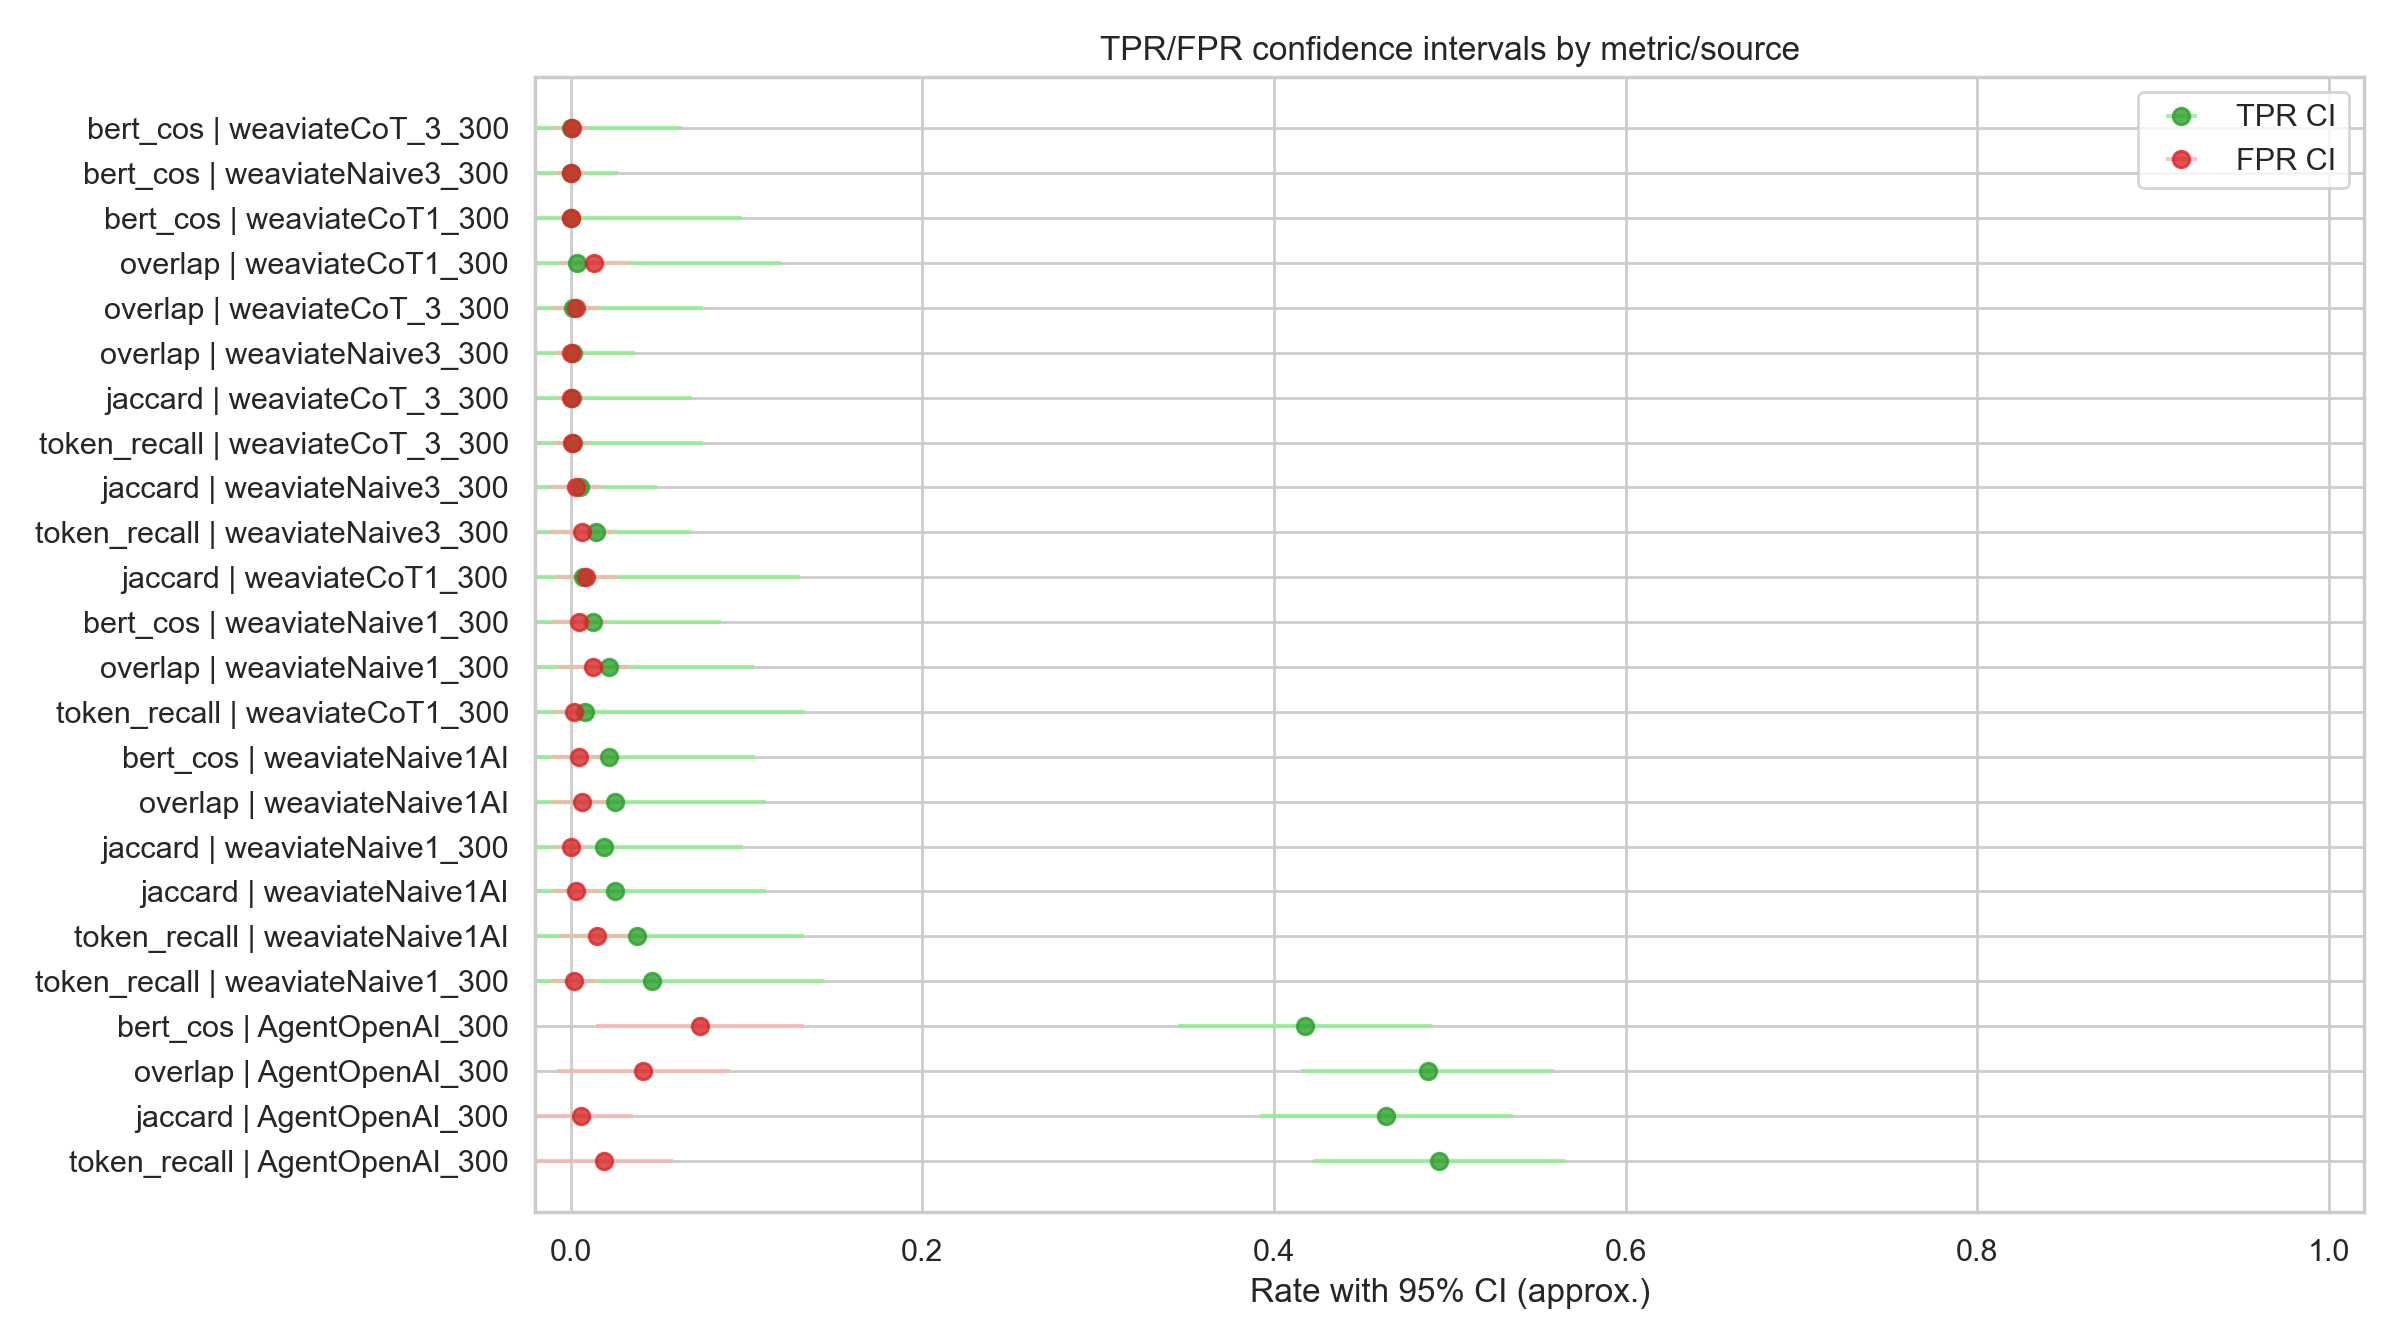
\includegraphics[width=1\linewidth]{Figures/06_tpr_fpr_confidence_intervals.png}
    \caption{confidence intervals for TPR and FPR per metric, for all source benchmark results, using the threshold that maximizes Youden's J statistic.}\label{fig:confidence-intervals}
\end{figure}

From the TPR and FPR confidence intervals (Figure~\ref{fig:confidence-intervals}), it can be observed that results benchmarked from the agentic RAG system have much better quality than the naive RAG system across all metrics. This indicates that the best benchmark for determining thresholds using Youden's J statistic is the agentic RAG system. One contributing factor is its more balanced behavior on missed and true retrievals. As seen from the document retrieved percentages shown in Table~\ref{tab:doc-retrieved-by-source}, the agentic RAG system substantially outperforms naive baselines: it correctly retrieves documents 60.4\% of the time, compared to 13.8\%–22.5\% for naive approaches and 5.7\%–9.4\% for chain-of-thought variants. This substantial improvement reflects the agent's ability to reason and plan, whereas the naive RAG system performs a single hybrid search.

\begin{table}[htbp]
    \centering
    \begin{tabular}{l c}
        \hline
        Source file & Correct document retrieved \\
        \hline
    AgentOpenAI\_300 & 60.4\% \\
    weaviateNaive3\_300 & 22.5\% \\
    weaviateNaive1\_300 & 13.8\% \\
    weaviateNaive1AI & 13.4\% \\
    weaviateCoT\_3\_300 & 9.4\% \\
    weaviateCoT1\_300 & 5.7\% \\
        \hline
    \end{tabular}
    \caption{Document retrieved percentage by source file}\label{tab:doc-retrieved-by-source}
\end{table}

\begin{table}[htbp]
  \centering
  \begin{tabular}{l c c c c}
    \hline
    Metric & Threshold & TPR & FPR & J \\
    \hline
    token\_recall & 0.67 & 56.7\% & 4.4\%  & 52.3\% \\
    jaccard       & 0.26 & 53.7\% & 2.0\%  & 51.7\% \\
    rouge1\_f     & 0.40 & 52.3\% & 2.7\%  & 49.7\% \\
    overlap       & 0.56 & 56.0\% & 7.7\%  & 48.3\% \\
    bleu          & 0.37 & 39.3\% & 1.3\%  & 37.9\% \\
    bert\_cos     & 0.71 & 49.0\% & 12.1\% & 36.9\% \\
    \hline
  \end{tabular}
    \caption{Best thresholds by metric (max True--False pass-rate difference) for File: AgentOpenAI\_300}\label{tab:agentopenai300-best-thresholds}
\end{table}

Table~\ref{tab:agentopenai300-best-thresholds}

\subsection{Overall Metric Results}
From the last subsection, the analysis indicates that the best metric thresholds (by Youden's J statistic) are obtained from the agentic RAG system; those thresholds are therefore used to categorize answers as correct or incorrect across benchmarks. The analysis is also narrowed to the best naive RAG variant (weaviateNaive1\_300), using qwen2.5 and OpenAI models, and the agentic RAG system (AgentOpenAI\_300). The results are presented in Figure~\ref{fig:median-metric} and Table~\ref{tab:gain-loss-reference-median}. The median metric scores are also presented for reference.
\begin{figure}
    \centering
    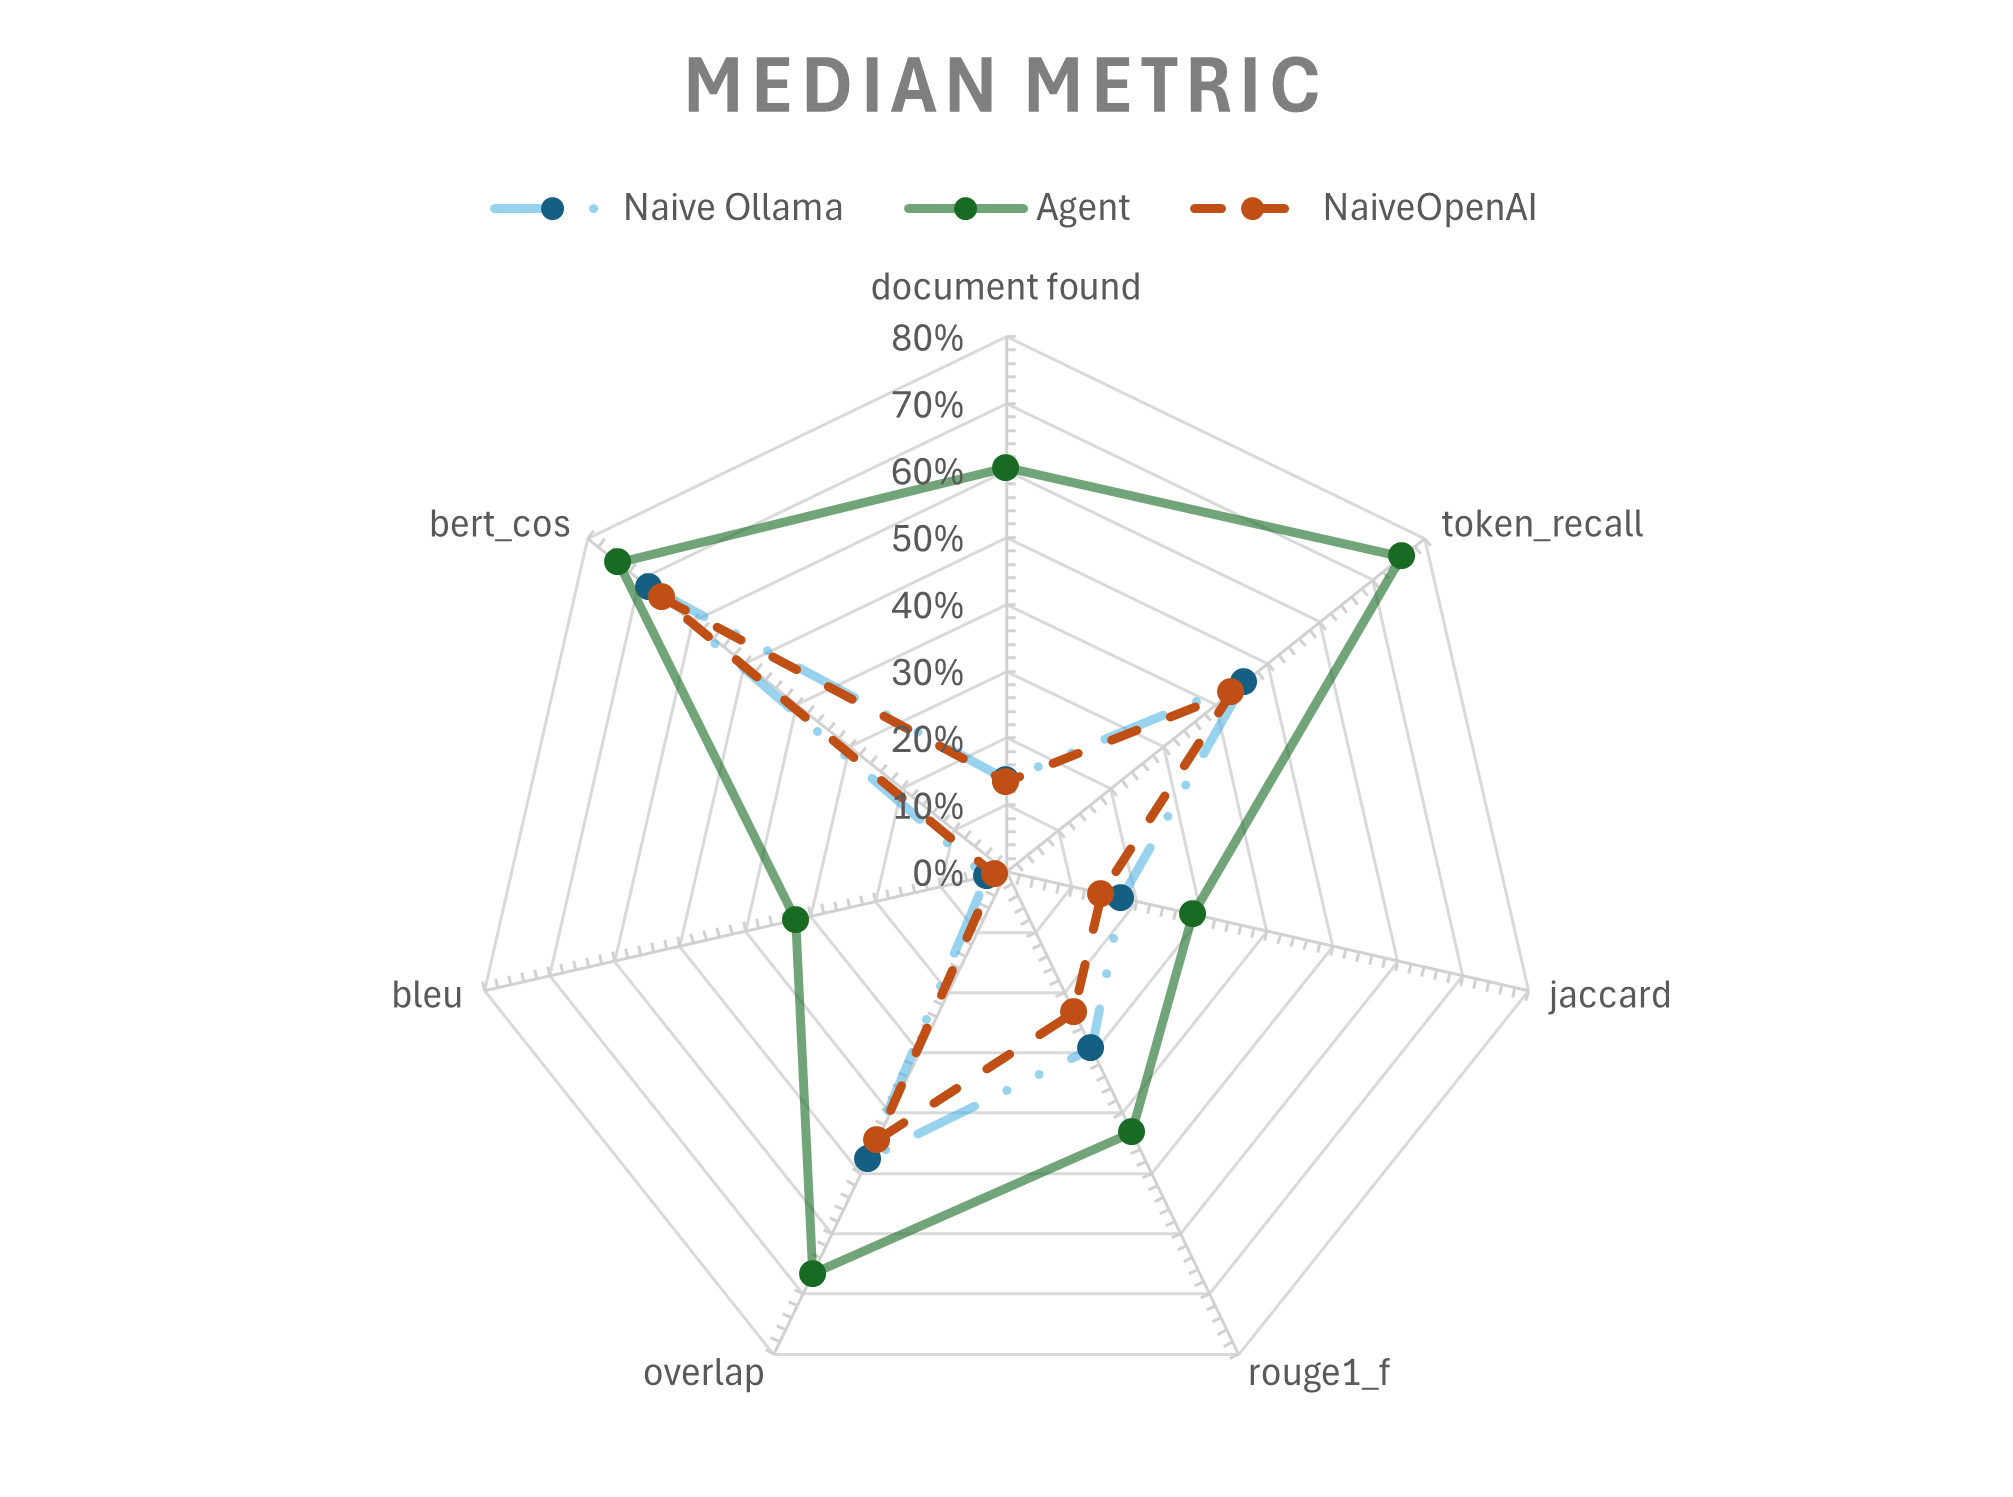
\includegraphics[width=0.75\linewidth]{Figures/Median Metric.png}
    \caption{Median Metric Scores}\label{fig:median-metric}
\end{figure}
According to Table~\ref{tab:agentopenai300-best-thresholds}, the metrics ranked by Youden's J statistic are: \textbf{Token Recall}, \textbf{Jaccard}, \textbf{ROUGE-1 F1}, \textbf{Overlap}, \textbf{BLEU}, and \textbf{\gls{BERT} cosine}. This ordering indicates which thresholds are most discriminative for correctly classifying answers as correct or incorrect in this dataset. Token Recall achieves the highest Youden's J value (52.3\%) because questions are specific and correctness hinges on including the right content words; surface fluency or paraphrase similarity is secondary. The -15\% trade-off observed in Table~\ref{tab:gain-loss-reference-median} reflects a deliberate threshold calibration: by optimizing for precision-oriented metrics (Jaccard, ROUGE-1), Token Recall is sacrificed slightly to avoid false positives, resulting in better overall classification balance. Conversely, \gls{BERT} cosine, which emphasizes sentence-level semantic proximity, performs worst here because many gold answers are short and exactness is required. Jaccard also performs well by rewarding coverage of relevant tokens relative to the union, providing a useful proxy for answer completeness.

\begin{table}[htbp]
    \centering
    \begin{tabular}{l r r r  r r r}
        \hline
        Approach &  token recall & jaccard & rouge1 & overlap & bleu & \gls{BERT} cosine \\
        \hline
        Agentic ReAct (\gls{GPT}-5) &  -15\% & 27\% & 12\% & -3\% & 8\% & -13\% \\
        Naive \gls{RAG} (\gls{GPT}-5) &  -31\% & -1\% & -9\% & -16\% & 1\% & -38\% \\
        Naive \gls{RAG} (Qwen2.5) &  -26\% & 5\% & -8\% & -9\% & -1\% & -30\% \\
        \hline
    \end{tabular}
    \caption{Numerical differences when using agentic reference thresholds (Youden-optimized)\ref{fig:Youden-metric} versus median-based \ref{fig:median-metric} thresholds for classifying answers (positive values indicate gains).}
    \label{tab:gain-loss-reference-median}
\end{table}

Applying the agentic reference thresholds yields clear gains for \textit{Agent OpenAI} on \textit{Jaccard} (+27\%), \textit{ROUGE-1} (+12\%), and \textit{BLEU} (+8\%), with a trade-off in \textit{Token Recall} (\textminus 15\%). \textit{\gls{BERT} cosine} declines (\textminus 13\%) are expected given the stricter, token-accuracy oriented thresholding. The naive baselines exhibit broad declines—especially in \textit{Token Recall} and \textit{\gls{BERT} cosine}—indicating that thresholds calibrated on higher-quality, better-retrieved agentic outputs do not transfer as well to weaker systems.
\begin{figure}
    \centering
    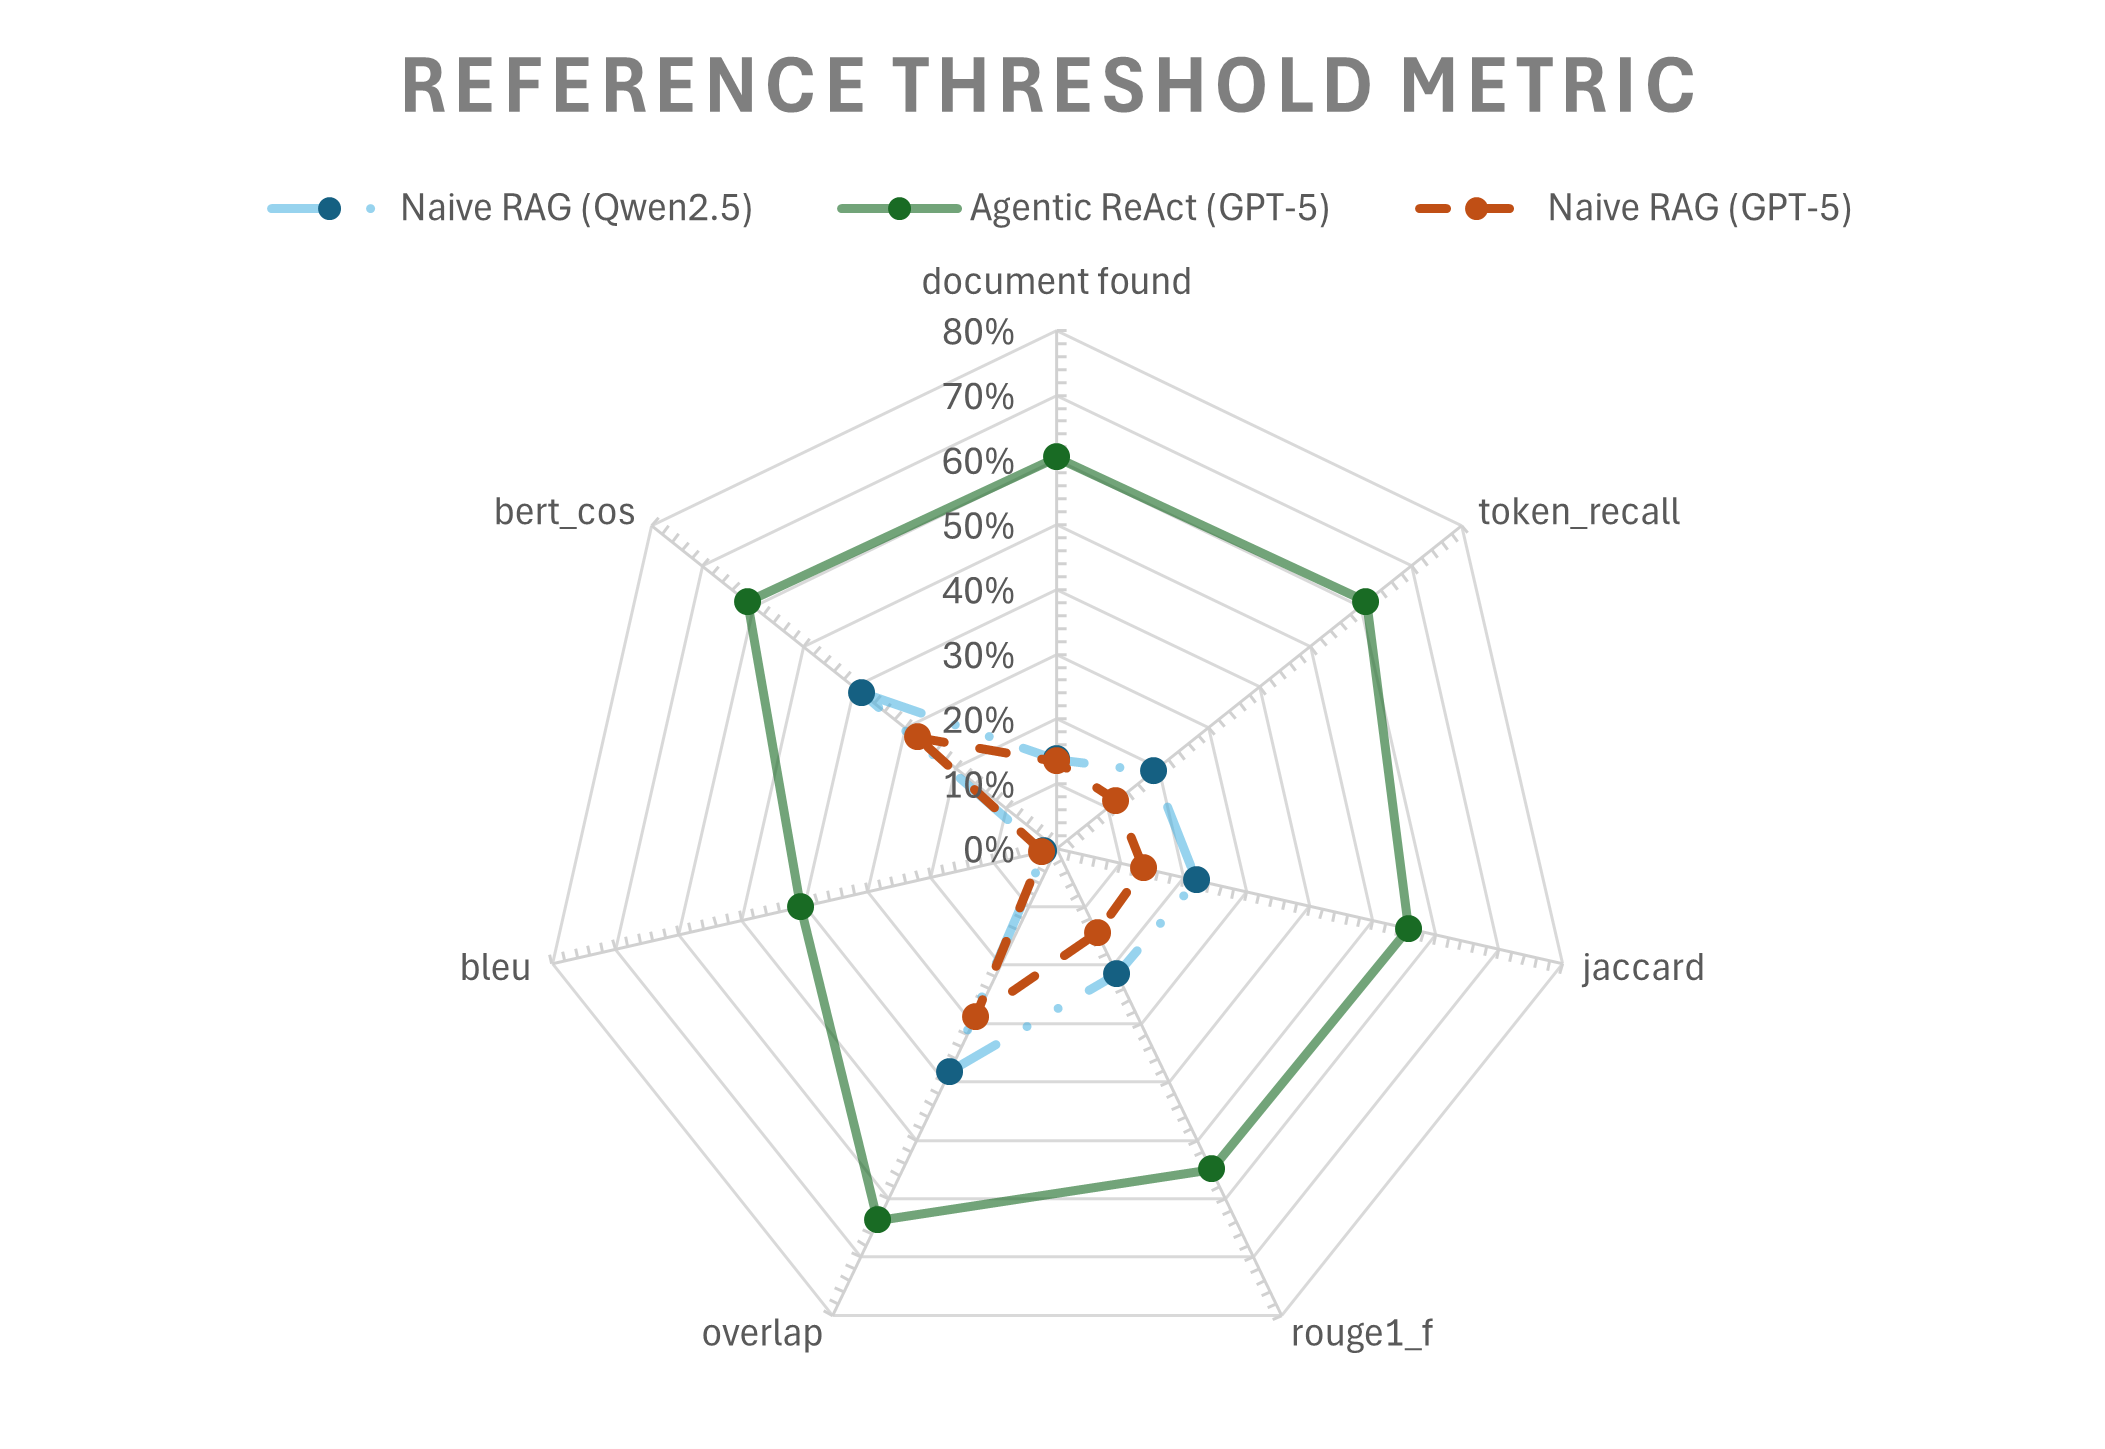
\includegraphics[width=0.75\linewidth]{Figures/Reference Threshold Metric.png}
    \caption{Agentic AI reference thresholds applied to all metrics of all important benchmarks}\label{fig:Youden-metric}
\end{figure}

Compared to the median-based thresholds, the agentic reference thresholds yield a more favorable profile for the \textit{Agent OpenAI} benchmark, boosting precision-oriented metrics (\textit{Jaccard}, \textit{ROUGE-1}, \textit{BLEU}) while sacrificing some recall (\textit{Token Recall}), but still remains a high score. This reflects the agent's ability to retrieve and synthesize relevant information more accurately, even if it occasionally omits less critical details. The naive baselines, however, do not benefit from this calibration, as their lower-quality outputs are less aligned with the stricter criteria derived from the agentic system.

\begin{table}[htbp]
    \centering
    \begin{tabular}{l r r r r r r}
        \hline
        Approach & token\_recall & jaccard & rouge1\_f & overlap & bleu & \gls{BERT} cosine \\
        \hline
        Agentic ReAct (\gls{GPT}-5) & 61\% & 56\% & 55\% & 64\% & 41\% & 61\% \\
        Naive \gls{RAG} (\gls{GPT}-5) & 12\% & 14\% & 14\% & 29\% & 2\% & 28\% \\
        Naive \gls{RAG} (Qwen2.5) & 19\% & 22\% & 21\% & 38\% & 2\% & 39\% \\
        \hline
    \end{tabular}
    \caption{Share of answers passing Youden-optimized thresholds (Figure~\ref{fig:Youden-metric})}
    \label{tab:youden-metric-values}
\end{table}

Taken together with Figure~\ref{fig:Youden-metric}, these values show a pronounced separation between the agentic system and naive baselines under Youden-optimized criteria. The \textit{Agent OpenAI} workflow—plan, retrieve, observe/reflect, and answer—consistently classifies a much larger fraction of outputs as correct across metrics (e.g., 61\% Token Recall and 64\% Overlap), whereas naive pipelines lag substantially (e.g., Token Recall 12–19\%, Overlap 29–38\%). This evidences the benefit of iterative reasoning and refinement over a single-pass naive RAG. This is also coupled by the fact that agentic RAG retrieves more documents correctly than the naive RAG system, as seen in Table~\ref{tab:doc-retrieved-by-source}.

\subsection{Cost and Latency Trade-offs}

Table~\ref{tab:naive-vs-agentic-tradeoffs} summarizes the cost and performance trade-offs between naive and agentic \gls{RAG} approaches. While naive \gls{RAG} is faster and cheaper (single retrieval + generation pass), agentic systems incur higher costs due to multiple reasoning and retrieval cycles. However, the significantly improved retrieval rate (60.4\% vs. 13.4\%–13.8\%) and answer quality justify this trade-off for mission-critical retrieval tasks.

\begin{table}[htbp]
    \centering
    \begin{tabular}{l r r r}
        \hline
        Approach & \gls{LLM} Calls/Query & Total Cost (300 Q) & Avg. Retrieval Rate \\
        \hline
        Naive \gls{RAG} (Qwen2.5) & 1--2 & 0 & 13.8\% \\
        Naive \gls{RAG} (\gls{GPT}-5) & 1--2 & \$5.07 & 13.4\% \\
        Agentic ReAct (\gls{GPT}-5) & 5--20 & \$18.35 & 60.4\% \\
        \hline
    \end{tabular}
    \caption{Comparative analysis of cost, latency, and retrieval effectiveness between naive and agentic \gls{RAG} approaches. Agentic systems require more \gls{LLM} calls but achieve substantially higher retrieval accuracy.}
    \label{tab:naive-vs-agentic-tradeoffs}
\end{table}

\section{Agentic Retrieval Across Multiple Collections}
\label{sec:agentic-retrieval-multiple}
In this experiment, the effectiveness of using multiple collections in Weaviate is evaluated and it is determined whether the agentic RAG system from Section~\ref{sec:agentic-test} can find information when it is distributed across different collections. The goal is to assess whether the agent can effectively navigate multiple data sources.

This is relevant in real-world scenarios where company information is spread across separate databases or collections organized by department, project, or document type. For example, a media publisher may purchase content feeds from multiple providers. Each provider might expose its catalog through a Weaviate instance and sell API access rather than delivering raw data. With a successful agentic RAG system, the publisher can issue a single query across these sources, retrieve the most relevant passages, and produce grounded answers for a news article.

To test this, two collections were set up in Weaviate. One is the collection used in the previous experiment (Section~\ref{sec:expNaiveVsAgenticRAG}), containing 1000 synthetic company documents. The second collection contains the LiHua-World dataset (Section~\ref{subsec:LiHua-World}).

For the \gls{QA} dataset, the 300 questions from the previous experiment (Section~\ref{sec:expNaiveVsAgenticRAG}) were combined with single-type questions from the LiHua-World dataset (637 in total) to match the synthetic setup. To avoid collection bias and control cost, 200 random questions were sampled from each dataset, yielding 400 questions overall. The total cost was 13.56 dollars for input tokens and 3.11 dollars for output tokens, totaling 16.67 dollars.

With this test, results were stored in \texttt{Agent\_OpenAI\_Mixed} and compared to the previous single-collection experiment \texttt{Agent\_OpenAI\_300}. Two split variants of the mixed dataset are also reported: \texttt{Agent\_OpenAI\_MixedLiHua} (LiHua-World questions only) and \texttt{Agent\_OpenAI\_MixedSynthetic} (synthetic company questions only).

To analyze the results, the percentage of questions for which the correct source document was retrieved is first examined, grouped by source file (Table~\ref{tab:doc-retrieved-by-source-mixed}). The mixed setting achieves higher retrieval rates than the single-collection setup. Part of this gain likely reflects random variation in the sampled questions; notably, even the \emph{MixedSynthetic} split outperforms the single-collection setup. Despite potential sampling effects, the results show that the agent performs robustly when retrieving across multiple collections.
\begin{table}[htbp]
    \centering
    \begin{tabular}{l c}
        \hline
        Approach & Avg. Retrieval Rate \\
        \hline
    Agent\_OpenAI\_MixedLiHua & 93.0\% \\
    Agent\_OpenAI\_Mixed & 86.0\% \\
    Agent\_OpenAI\_MixedSynthetic & 80.5\% \\
    Agent\_OpenAI\_300 & 60.4\% \\
        \hline
    \end{tabular}
    \caption{Share of questions with the correct document retrieved, by result file}\label{tab:doc-retrieved-by-source-mixed}
\end{table}

\section{Optimization Using Summarization}
To optimize retrieval and generation performance, text summarization techniques were applied to the document corpus before indexing in Weaviate. The goal was to reduce document length while preserving essential information, enabling more efficient embedding and retrieval.
This is particularly important for long documents where embedding models may truncate input or dilute semantic focus.
Two summarization approaches tested are LexRank and BART-based abstractive summarization (see Section~\ref{sec:text-summarization} for details).
The original synthetic company documents (1000 files) were summarized using both techniques, producing two new corpora: \texttt{Synthetic\_LexRank} and \texttt{Synthetic\_BART}. The source path to the unsummarized documents was retained for grounding answers in to the Weaviate database.
Each summarized corpus was indexed in separate Weaviate collections using the same schema as before (class \textit{Ficheiro} with properties \texttt{text} and \texttt{file\_path}, vectorized with \textit{all-MiniLM-L6-v2} embeddings). The agentic RAG system from Section~\ref{sec:agentic-test} was not evaluated because of budget contraints, and what is tested is the impact of summarization with the purpose of optimizing storage, and denoising the database, for more efficient embedding and retrieval. Which is only required comparison between the naive RAG system from Section~\ref{sec:naive-rag-and-cot-baseline}.
Each summarization approach was evaluated by running the naive RAG pipeline (using \texttt{qwen2.5m} for generation) on the same 300-question benchmark from Section~\ref{sec:expNaiveVsAgenticRAG}. 

To take advantage of previous results, it is used the best-performing naive RAG variant from Section~\ref{sec:naive-rag-and-cot-baseline} as a baseline: \texttt{weaviateNaive1\_300} (using hybrid search with \(\alpha=0.7\) and top-1 retrieval). And the same evaluation metrics from Section~\ref{sec:metric-evaluation-quality}, the Youden's statistic metric thresholds from the most balanced benchmark, \texttt{Agentic React (\gls{GPT}-5)} are applied to compare performance across the three approaches: original, LexRank-summarized, and BART-summarized. The most important Youden's metric analyzed are \textbf{Token Recall}, and \textbf{Jaccard}, which are used in to best reflect the ability to retrieve the correct document and generate accurate answers in this experiment.
The results are presented in table~\ref{tab:document_retrieved_metrics_summarization}.

\begin{table}[t]
\centering
\caption{Document retrieval and summarization metrics}
\label{tab:document_retrieved_metrics_summarization}
\begin{tabular}{lrrr}
\hline
Approach & Avg. Retrieval Rate & token recall & jaccard \\
\hline
Agentic ReAct (\gls{GPT}-5)& 60.4\% & 61.1\%  & 55.7\%\\
LexRank & 33.6\% & 29.5\%  & 35.9\% \\
BART & 17.8\% & 3.0\% & 11.1\% \\
Naive \gls{RAG} (Qwen2.5) & 13.8\% & 19.1\% & 22.1\% \\
\hline
\end{tabular}
\end{table}

The results show that summarization techniques help reduce noise in the \gls{VD}, as Avg. Retrieval Rate increased in both summarization approaches compared to the naive RAG baseline (13.8\%): LexRank achieved 33.6\% and BART 17.8\%.
LexRank also improved Token Recall and Jaccard scores (29.5\% and 35.9\%, respectively), indicating that the extractive summaries preserved key information needed for accurate answering.
However, in the case of BART, the Token Recall and Jaccard scores were significantly lower (3.0\% and 11.1\%, respectively), indicating that while retrieval improved, the generated answers were less accurate. This suggests that BART's abstractive summarization may have omitted critical information needed for precise answering.
With this results, it is concluded that summarization of documents is a valuable step in a \gls{RAG} pipeline, functioning as a filter to reduce noise (irrelevant content).
However, the choice of summarization technique need to be carefully considered: extractive methods like LexRank appear more effective as they preserve essential details, while abstractive methods like BART risk losing important details.

% Finally, the summarization techniques were also evaluated in the mixed dataset from Section~\ref{sec:agentic-retrieval-multiple}, combining both LiHua-World and synthetic company questions. The same naive RAG pipeline (using \texttt{qwen2.5m} for generation) was run on the mixed 400-question benchmark, using the same Weaviate collections with summarized documents. In this case the collections were merged in to one, as the decision making of a agent is not relevant in this experiment. The goal of this experiment, is evaluating the impact of summarization techniques in a mixed dataset scenario.

% The results are presented in table~\ref{tab:document_retrieved_metrics_mixed}.
% \begin{table}[t]
% \centering
% \caption{Document retrieval and summarization metrics using mixed dataset from Section~\ref{sec:agentic-retrieval-multiple}}
% \label{tab:document_retrieved_metrics_mixed}
% \begin{tabular}{lrrr}
% \hline
% Approach & Avg. Retrieval Rate & token recall & jaccard \\
% \hline
% MixedLiHua & 46.5\% & 15.8\% & 1.27\% \\
% MixedTotal & 39.4\% & 24.6\% & 19.3\% \\
% LexRank & 33.6\% & 29.5\%  & 35.9\% \\
% MixedSynthetic & 33.0\% & 31.5\% & 33.5\% \\
% \hline
% \end{tabular}
% \end{table}

% The results show that summarization techniques need to be carefully considered. As the Lihua-World benchmark, Avg. Retrieval Rate is high, the answer quality is poor. This happens because the Lihua-World dataset, is dialogues snippets, of a fictional story. Where details are more hidden. Therefore, LexRank summarization ended up removing 